 
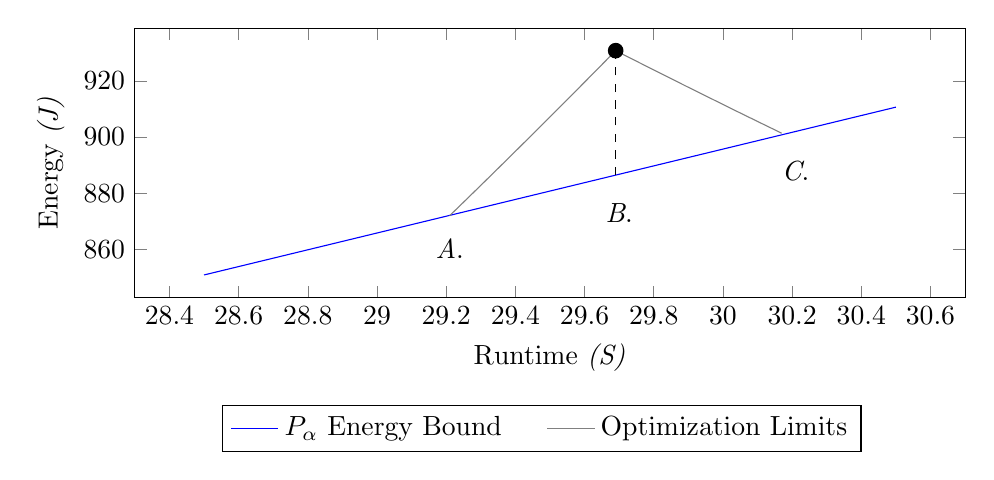
\begin{tikzpicture}
  \begin{axis}[no markers, ylabel={Energy \emph{(J)}}, xlabel={Runtime \emph{(S)}}, axis on top,
    width=\linewidth,
    height=5cm,
    legend style={at={(0.49,-0.4)}, anchor=north,legend columns=2, /tikz/every even column/.append style={column sep=0.5cm}}
    ]

    \pgfmathsetmacro{\baseline}{29.857} % NOP code

    %code, power, time
    %cfd, 31.348872, 29.689872
    %heartwall, 32.072718, 24.456485
    %lavaMD,  32.715703, 65.387028
    %leukocyte, 30.771108, 38.950881
    %streamcluster, 32.192283, 33.801999


     \addplot[domain=28.5:30.5, blue] {\baseline * x};
     \addlegendentry{$P_{\alpha}$ Energy Bound} 

  
     %% CFD %%
     \pgfmathsetmacro{\cfdpower}{31.348872}
     \pgfmathsetmacro{\cfdtime}{29.689872}
     \pgfmathsetmacro{\cfdenergy}{\cfdpower * \cfdtime}
     \pgfmathsetmacro{\baseenergy}{\baseline * \cfdtime}
     \addplot[domain=\cfdtime:30.17, gray, forget plot] { (\cfdpower * \cfdtime^3) / ((x)^2)};
     \addplot[domain=29.21:\cfdtime, gray] { (\cfdpower / \cfdtime^3) * x^4}; % Power time same ratio

     \node[circle,fill,inner sep=2pt] at (axis cs:\cfdtime, \cfdenergy) {};
     \addlegendentry{Optimization Limits} 

    \draw[dashed] ({axis cs:\cfdtime,0}|-{axis cs:0,\baseenergy}) -- ({axis cs:\cfdtime,0}|-{axis cs:0,\cfdenergy});
    
    \node at (axis cs:29.21,860) {\textit A.};                                   
    \node at (axis cs:29.7,873) {\textit B.};                                   
    \node at (axis cs:30.21,888) {\textit C.};                                   



%     %% CFD %%
%     \addplot[domain=39:48, gray] { (\sedtargetenergy * \sedtargetseconds *  \sedtargetseconds) / ((x)^2)};
%     \addplot[domain=33:41, gray] { (\sedtargetpower / \sedtargetseconds^3) * x^4}; % Power time same ratio
%     \addlegendentry{$ED^{2}P$} 
 

    
      
 \end{axis}
\end{tikzpicture}
